%
% This is the LaTeX template file for lecture notes for CS5234,
% Algorithms at Scale.  When preparing 
% LaTeX notes for this class, please use this template.
%
% To familiarize yourself with this template, the body contains
% some examples of its use.  Look them over.  Then you can
% run LaTeX on this file.  After you have LaTeXed this file then
% you can look over the result either by printing it out with
% dvips or using xdvi.
%
% This template is based on the template at https://inst.eecs.berkeley.edu/~cs294-8/sp03/Materials/scribe.tex.

\documentclass[twoside]{article}
\usepackage{graphics}
\usepackage{amsmath}
\usepackage{amsfonts}
\usepackage[utf8]{inputenc}
\usepackage{tikz}
\usepackage[tight,footnotesize]{subfigure}

\usetikzlibrary{arrows.meta}
\usetikzlibrary{arrows, automata, positioning, through}

\setlength{\oddsidemargin}{0.25 in}
\setlength{\evensidemargin}{-0.25 in}
\setlength{\topmargin}{-0.6 in}
\setlength{\textwidth}{6.5 in}
\setlength{\textheight}{8.5 in}
\setlength{\headsep}{0.75 in}
\setlength{\parindent}{0 in}
\setlength{\parskip}{0.1 in}

%
% The following commands set up the lecnum (lecture number)
% counter and make various numbering schemes work relative
% to the lecture number.
%
\newcounter{lecnum}
\renewcommand{\thepage}{\thelecnum-\arabic{page}}
\renewcommand{\thesection}{\thelecnum.\arabic{section}}
\renewcommand{\theequation}{\thelecnum.\arabic{equation}}
\renewcommand{\thefigure}{\thelecnum.\arabic{figure}}
\renewcommand{\thetable}{\thelecnum.\arabic{table}}
\renewcommand{\arraystretch}{2}
%
% The following macro is used to generate the header.
%
\newcommand{\lecture}[4]{
   \pagestyle{myheadings}
   \thispagestyle{plain}
   \newpage
   \setcounter{lecnum}{#1}
   \setcounter{page}{1}
   \noindent
   \begin{center}
   \framebox{
      \vbox{\vspace{2mm}
    \hbox to 6.28in { {\bf CS 5234 Algorithms at Scale
                        \hfill \today} }
       \vspace{4mm}
       \hbox to 6.28in { {\Large \hfill Lecture #1: #2  \hfill} }
       \vspace{2mm}
       \hbox to 6.28in { {\it Lecturer: #3 \hfill Scribe: #4} }
      \vspace{2mm}}
   }
   \end{center}
   \markboth{Lecture #1: #2}{Lecture #1: #2}
   {\bf Disclaimer}: {\it These notes have not been subjected to the
   usual scrutiny reserved for formal publications.  They may be distributed
   outside this class only with the permission of the Instructor.}
   \vspace*{4mm}
}

%
% Convention for citations is authors' initials followed by the year.
% For example, to cite a paper by Leighton and Maggs you would type
% \cite{LM89}, and to cite a paper by Strassen you would type \cite{S69}.
% (To avoid bibliography problems, for now we redefine the \cite command.)
% Also commands that create a suitable format for the reference list.
\renewcommand{\cite}[1]{[#1]}
\def\beginrefs{\begin{list}%
        {[\arabic{equation}]}{\usecounter{equation}
         \setlength{\leftmargin}{2.0truecm}\setlength{\labelsep}{0.4truecm}%
         \setlength{\labelwidth}{1.6truecm}}}
\def\endrefs{\end{list}}
\def\bibentry#1{\item[\hbox{[#1]}]}

%Use this command for a figure; it puts a figure in wherever you want it.
%usage: \fig{NUMBER}{SPACE-IN-INCHES}{CAPTION}
\newcommand{\fig}[3]{
			\vspace{#2}
			\begin{center}
			Figure \thelecnum.#1:~#3
			\end{center}
	}
% Use these for theorems, lemmas, proofs, etc.
\newtheorem{theorem}{Theorem}[lecnum]
\newtheorem{lemma}[theorem]{Lemma}
\newtheorem{proposition}[theorem]{Proposition}
\newtheorem{claim}[theorem]{Claim}
\newtheorem{corollary}[theorem]{Corollary}
\newtheorem{definition}[theorem]{Definition}
\newenvironment{proof}{{\bf Proof:}}{\hfill\rule{2mm}{2mm}}

% **** IF YOU WANT TO DEFINE ADDITIONAL MACROS FOR YOURSELF, PUT THEM HERE:

\begin{document}
%FILL IN THE RIGHT INFO.
%\lecture{**LECTURE-NUMBER**}{**DATE**}{**LECTURER**}{**SCRIBE**}
\lecture{3}{Markov Chain Monte Carlo}{Arnab Bhattacharyya}{Jiun Wei, Changsheng, Yuchen, Shawn}
%\footnotetext{These notes are partially based on those of Nigel Mansell.}

% **** YOUR NOTES GO HERE:

% Scribe: Jiun Wei
\section{Introduction}

Recall that in the last lecture, we saw sampling applied to:

\begin{enumerate}
   \item Approximate Counting
   \item Bayesian Inference
\end{enumerate}

For approximate counting, we wanted to uniformly sample from the space of valid solutions to a computational problem (e.g., the 0-1 Knapsack Problem).

For Bayesian inference, we wanted to sample from a posterior distribution $P$ such that:
\[
P(x) = \frac{f(x)}{Z}
\]
where $f(x)$ is known but $Z$ is unknown.

\subsection{Markov Chain Monte Carlo}

Both sampling tasks can be accomplished using a method called Markov Chain Monte Carlo (MCMC).

Suppose \(P\) is the target distribution that we wish to sample from over $\Omega$, the universe of all possible states.

The main idea is that we start from a known state $X_0$ at $t = 0$ in $\Omega$ and make random transitions to $X_1$ at $t = 1$, $X_2$ at $t = 2$, $X_3$ at $t = 3$ and so on. Each transition to the next state is also based solely on the current state and not on the previous states that came before.

For MCMC, we want that for large $t$, $Pr[X_t = x] \approx P(x)$.

Assuming certain conditions are met, the sequence of $X_0, X_1, X_2$ and so on is called a Markov Chain.

\begin{definition}[Markov Chain]
   A Markov Chain over $\Omega$ is a sequence of random variables $X_0, X_1, X_2, ...$ such that:
   \begin{enumerate}
      \item $\forall t, X_t$ takes values in $\Omega$.
      \item $\forall x_0, x_1, ..., x_{t+1} \in \Omega: Pr[X_{t+1} = x_{t+1}|X_0 = x_0, X_1 = x_1, ..., X_t = x_t] = Pr[X_{t+1} = x_{t+1}|X_t = x_t]$ \\
      (Informally: the next move only depends on current state, not past history.)
      \item $Pr[X_{t+1} = y|X_t = x] = M(x, y)$ is independent of $t$.
   \end{enumerate}
\end{definition}

The last point also allows us to formulate an $|\Omega| \times |\Omega|$ transition matrix $M$.

\subsection{Example: Card Shuffling}

We can think of multiple card shufflings as a Markov Chain where each permutation or ordering of the standard 52 cards in a deck constitutes a state. Card shuffling is a random process, and we hope that after enough shuffles, the deck is equally likely to be any of the states in $\Omega$, where $\Omega$ = all possible ordering of the cards (i.e., $|\Omega| = 52!$). This was also demonstrated using the Jupyter notebook via simulated riffle shuffles.


% Scribe: Changsheng
% Scribe: Changsheng
\section{Stationary Distributions}

\subsection{Example: Finite State Machine}
Markov chains can be represented by finite state machines. The idea is that a Markov chain describes a process in which the transition to a state at time $t+1$ depends only on the state at time $t$. The main thing to keep in mind is that the transitions in a Markov chain are probabilistic rather than deterministic, which means that you can't always say with perfect certainty what will happen at time $t+1$.

This Markov Chain usually shown by a \textbf{state transition diagram}. Consider a Markov chain with three possible states $0, 1$ and $2$, i.e. $\Omega = \{0,1,2\}$ and the following transition probabilities.

\begin{equation}\mathbf{P}_r=\left[\begin{array}{ccc}
\frac{1}{2} & \frac{1}{4} & \frac{1}{4} \\
\frac{1}{4} & \frac{1}{2} & \frac{1}{4} \\
\frac{1}{4} & \frac{1}{4} & \frac{1}{2}
\end{array}\right]\end{equation}

the state transition diagram can be drawn as,

\begin{figure}[!htp]
	\centering
		\label{fig:fs_machine}
		\begin{tikzpicture}[->,>=stealth',shorten >=1pt,auto,node distance=4cm,
                thick,main node/.style={circle,draw,font=\Large\bfseries}]

        \node[main node] (0) {0};
        \node[main node] (1) [below left of=0] {1};
        \node[main node] (2) [below right of=0] {2};

          \path
            (0) edge    [loop above]    node            {$\frac{1}{2}$} (0)
                edge                    node            {$\frac{1}{4}$} (1)
                edge    [bend left]     node            {$\frac{1}{4}$} (2)
            (1) edge    [loop below]    node            {$\frac{1}{2}$} (1)
            	edge    [bend left]     node            {$\frac{1}{4}$} (0)
                edge    [bend right]    node            {$\frac{1}{4}$} (2)
            (2) edge    [loop below]    node            {$\frac{1}{2}$} (2)
                edge                    node    [above] {$\frac{1}{4}$} (1)
                edge                    node            {$\frac{1}{4}$} (0);
\end{tikzpicture}
	\caption{This graph shows an example of a finit state machine with 3 states. The edges denote the  transition probabilities.}
\end{figure}


\begin{figure}[!t]
   \centering
	\subfigure[$t=0$ \textbf{Initial State}]{
		\label{fig:t0}
		\begin{tikzpicture}[->,>=stealth',shorten >=1pt,auto,node distance=2cm, thick,main node/.style={circle,draw,font=\bfseries}]

        \node[main node] (0)                    {$1$};
        \node[main node] (1) [below left of=0]  {$0$};
        \node[main node] (2) [below right of=0] {$0$};

          \path
            (0) edge [loop above]   node                {}  (0)
                edge                node                {}  (1)
                edge [bend left]    node                {}  (2)
            (1) edge [loop below]   node                {}  (1)
            	edge [bend left]    node                {}  (0)
                edge [bend right]   node                {}  (2)
            (2) edge [loop below]   node                {}  (2)
                edge                node    [above]     {}  (1)
                edge                node                {}  (0);
        \end{tikzpicture}
	}
   \subfigure[$t=1$]{
		\label{fig:t1}
		\begin{tikzpicture}[->,>=stealth',shorten >=1pt,auto,node distance=2cm, thick,main node/.style={circle,draw,font=\bfseries}]

        \node[main node] (0)                    {$\frac{1}{2}$};
        \node[main node] (1) [below left of=0]  {$\frac{1}{4}$};
        \node[main node] (2) [below right of=0] {$\frac{1}{4}$};

          \path
            (0) edge [loop above]   node                {}  (0)
                edge                node                {}  (1)
                edge [bend left]    node                {}  (2)
            (1) edge [loop below]   node                {}  (1)
            	edge [bend left]    node                {}  (0)
                edge [bend right]   node                {}  (2)
            (2) edge [loop below]   node                {}  (2)
                edge                node    [above]     {}  (1)
                edge                node                {}  (0);
        \end{tikzpicture}
   }
   \subfigure[$t=2$]{
		\label{fig:t2}
		\begin{tikzpicture}[->,>=stealth',shorten >=1pt,auto,node distance=2cm, thick,main node/.style={circle,draw,font=\bfseries}]

        \node[main node] (0)                    {$\frac{3}{8}$};
        \node[main node] (1) [below left of=0]  {$\frac{5}{16}$};
        \node[main node] (2) [below right of=0] {$\frac{5}{16}$};

          \path
            (0) edge [loop above]   node                {}  (0)
                edge                node                {}  (1)
                edge [bend left]    node                {}  (2)
            (1) edge [loop below]   node                {}  (1)
            	edge [bend left]    node                {}  (0)
                edge [bend right]   node                {}  (2)
            (2) edge [loop below]   node                {}  (2)
                edge                node    [above]     {}  (1)
                edge                node                {}  (0);
        \end{tikzpicture}
   }
   \subfigure[$t=3 \rightarrow t=n$]{
        \label{fig:t3}
        
		\begin{tikzpicture}[->,>=stealth',shorten >=1pt,auto,node distance=2cm, thick,main node/.style={circle,draw,font=\bfseries}]    
        \node[main node] (0)                    {$\frac{22}{64}$};
        \node[main node] (1) [below left of=0]  {$\frac{21}{64}$};
        \node[main node] (2) [below right of=0] {$\frac{21}{64}$};

          \path
            (0) edge [loop above]   node                {}  (0)
                edge                node                {}  (1)
                edge [bend left]    node                {}  (2)
            (1) edge [loop below]   node                {}  (1)
            	edge [bend left]    node                {}  (0)
                edge [bend right]   node                {}  (2)
            (2) edge [loop below]   node                {}  (2)
                edge                node    [above]     {}  (1)
                edge                node                {}  (0);
        \end{tikzpicture}
        
        
        \centering
        $\cdots$
        % \centering
        % $\cdots$

        \begin{tikzpicture}[->,>=stealth',shorten >=1pt,auto,node distance=2cm, thick,main node/.style={circle,draw,font=\bfseries}]

            \node[main node] (0)                    {$\approx \frac{1}{3}$};
            \node[main node] (1) [below left of=0]  {$\approx \frac{1}{3}$};
            \node[main node] (2) [below right of=0] {$\approx \frac{1}{3}$};
    
              \path
                (0) edge [loop above]   node                {}  (0)
                    edge                node                {}  (1)
                    edge [bend left]    node                {}  (2)
                (1) edge [loop below]   node                {}  (1)
                    edge [bend left]    node                {}  (0)
                    edge [bend right]   node                {}  (2)
                (2) edge [loop below]   node                {}  (2)
                    edge                node    [above]     {}  (1)
                    edge                node                {}  (0);
            \end{tikzpicture}
   }
   \subfigure[\textbf{Stationary}]{
		\label{fig:stationary}
		\begin{tikzpicture}[->,>=stealth',shorten >=1pt,auto,node distance=2cm, thick,main node/.style={circle,draw,font=\bfseries}]

        \node[main node] (0)                    {$\frac{1}{3}$};
        \node[main node] (1) [below left of=0]  {$\frac{1}{3}$};
        \node[main node] (2) [below right of=0] {$\frac{1}{3}$};

          \path
            (0) edge [loop above]   node                {}  (0)
                edge                node                {}  (1)
                edge [bend left]    node                {}  (2)
            (1) edge [loop below]   node                {}  (1)
            	edge [bend left]    node                {}  (0)
                edge [bend right]   node                {}  (2)
            (2) edge [loop below]   node                {}  (2)
                edge                node    [above]     {}  (1)
                edge                node                {}  (0);
        \end{tikzpicture}
   }

	\caption{Above shows an example of the diffusion process of the above mentioned finite state machine. Suppose we start from state 0. In Figure \ref{fig:t0}, node $0$ has an initial probability value $1$ node $1$ and node $2$ have the initail value of $0$, and in the next state, e.g. we can compute the value of node $0$ by $\frac{1}{2} = \frac{1}{2} \cdot 1 + \frac{1}{4} \cdot 0 + \frac{1}{4} \cdot 0$. We can find that, with the $t$ advances and transition take place, the probability values of being at each state of all nodes start to converge to $\frac{1}{3}$ }
	\label{fig:s2tAndt2t}
\end{figure}


 We eventually find that the probability of being at each state converges to $\frac{1}{3}$. This is called a \textbf{Stationary Distribution} because the resulting probability values are no longer changed by application of the transition probabilities.

\begin{definition}[Stationary Distribution]
   $\pi$ is a stationary distribution if
   $$
   \forall y \in \Omega, \pi(y) = \sum_{x \in \Omega} \pi(x) \cdot M(x, y)
   $$
\end{definition}

\textbf{Question:} As $t \rightarrow \infty$, does the distribution of $X_t$ always converge to a stationary distribution?
\begin{figure}[!htp]
	\centering
		\label{fig:fs_machine}
		\begin{tikzpicture}[->,>=stealth',shorten >=1pt,auto,node distance=4cm,
                thick,main node/.style={circle,draw,font=\Large\bfseries}]

        \node[main node] (0) {A};
        \node[main node] (1) [right of=0] {B};

          \path
            (0)
                edge     [bend left]               node            {$1$} (1)
                
            (1)
            	edge    [bend left]     node            {$1$} (0);
                
\end{tikzpicture}
    \caption{An example of a 2-state system. In this system, $\pi = [\frac{1}{2} \ \frac{1}{2}]$ is stationary.}
\end{figure}

The answer is no. For instance, consider a 2-state system that always transitions to the other state with probability 1. In this case, no convergence is ever achieved as $t \rightarrow \infty$.

\begin{definition}[Regular]
   

A Markov Chain is \textbf{regular} if $\exists$ $T_0 > 0$ such that for any two states $x$ and $y$, there is a path of length $T_0$ from $x$ to $y$.

\end{definition}

\begin{theorem}
   A finite regular Markov Chain has a unique stationary distribution $\pi$ that it converges to if
   $$
   \forall x \in \Omega, \lim_{t \rightarrow \infty} Pr[X_t = x] = \pi(x)
   $$
\end{theorem}

All Markov Chains have stationary distributions, but not all converge to it.

\textbf{MCMC Strategy:}  Design a Markov chain whose stationary distribution is the one you want to sample from.

\begin{lemma}
   $\pi$ is a stationary distribution if it satisfies the ``detailed balance'' equation:
   $$
   \forall x,y: \pi(x) \cdot M(x, y) = \pi(y) \cdot M(y, x)
   $$
\end{lemma}

\begin{corollary}
   A Markov Chain has uniform stationary distribution if $M(x, y) = M(y, x)$ $\forall x, y$.
\end{corollary}






% Scribe: Yuchen
\section{Application to Knapsack Problem $KP(L)$}

\begin{itemize}
   \item Weights: $w_1,w_2, ..., w_n$
   \item Limit: $L$
   \item $\Omega$ = Solutions to KP(L)
   \item $X_0 = \emptyset$
\end{itemize}

And then we define the transition from t. Suppose we have $X_t$, and here is how we generate $X_{t+1}$.  

At step $t$, choose $i \in [n]$ uniformly at random.

$$
X_{t+1} = \begin{cases}
   X_t \setminus \{i\} & \text{if } i \in X_t \\
   X_t \cup \{i\} & \text{if } i \notin X_t \text{ and } \sum_{k \in X_t \cup \{i\}} w_k \leq L\\
   X_t & \text{otherwise}
\end{cases}
$$

We can easily check that this is regular. Firstly, check that we can go from any state to any other state, i.e. a path should exist. Secondly, there's a self-loop transition somewhere, i.e. $X_{t+1}=X_t$ for some states. Otherwise, we never violate the weights constrains, which means that $\sum_{k \in X_t \cup \{i\}} w_k \leq L $ will always be true.

According to Corollary \ref{knapsack}, this Markov Chain's transition probabilities from state $S$ to any adjacent state $S'$ and vice versa are the same at $M(S, S') = M(S', S) = \frac{1}{n}$. And the Markov Chain converges to a uniform stationary distribution. Hence, it is possible to sample uniformly from the population of KP(L) solutions using the MCMC method.

A question to think about (but won't be discussed in this class): The claimable convergence is $t \rightarrow \infty$, but we will only running the Markov Chain on a smaller number of sets. So how close do we get to the uniformly distribution?






% Scribe: Shawn
\section{Metropolis-Hastings}

Recall the Bayesian inference setup, where we want to generate samples from a distribution P, such that $P(x) = \frac{f(x)}{Z}, f: \Omega \rightarrow \mathbb{R}^{\geq 0}$. The function $f(x)$ can be thought of as a score that determines how desirable it is to be in state $x$, while $Z$ is some normalizing constant that is prohibitively expensive to compute. 

The Metropolis-Hastings algorithm allows us to design a Markov Chain with stationary distribution $P$, thus providing us with a method of sampling from $P$ without having to compute $Z$. Suppose you have a regular Markov Chain on $\Omega$ with transition matrix $M$. We define the Metropolis-Hastings Markov Chain transitions as follows:

\begin{enumerate}
   \item Pick $Y$ with probability $M(X_t, Y)$.
   \item Set $\alpha = \min\{ 1, \frac{P(Y) \cdot M(Y, X_t)}{P(X_t) \cdot M(X_t, Y)} \}$, using $\frac{P(Y)}{P(X)} = \frac{f(Y)}{f(X)}$
   \item With probability $\alpha$, $X_{t+1} \leftarrow Y$ and with probability $1 - \alpha$, $X_{t+1} \leftarrow X_t$.
\end{enumerate}

\begin{theorem}
  The stationary distribution $\pi$ of the Metropolis-Hastings Markov Chain is $P$
\end{theorem}

\begin{proof}
Let $M$ be the transition matrix of the original Markov chain, and let $Q$ be the transition matrix of the Metropolis-Hastings Markov chain. Then:

\begin{equation*}
\begin{split}
P(i) \cdot Q(i,j)  & = P(i) \cdot M(i,j) \cdot \mbox{min}\{1, \frac{P(j) \cdot M(j,i)}{P(i) \cdot M(i,j)}\} = \mbox{min}\{P(i) \cdot M(i,j), P(j) \cdot M(j,i) \} \\
& = P(j) \cdot M(j,i) \cdot \mbox{min}\{\frac{P(i) \cdot M(i,j)}{P(j) \cdot M(j,i)}, 1 \} = P(j) \cdot Q(j, i)
\end{split}
\end{equation*}

By the balance lemma, $P$ is the stationary distribution with respect to $Q$
\end{proof}

% \section*{References}
% \beginrefs
% \bibentry{AGM97}{\sc N.~Alon}, {\sc Z.~Galil} and {\sc O.~Margalit},
% On the Exponent of the All Pairs Shortest Path Problem,
% {\it Journal of Computer and System Sciences\/}~{\bf 54} (1997),
% pp.~255--262.

% \bibentry{F76}{\sc M. L. ~Fredman}, New Bounds on the Complexity of the 
% Shortest Path Problem, {\it SIAM Journal on Computing\/}~{\bf 5} (1976), 
% pp.~83-89.
% \endrefs


\end{document}



